\chapter{Eficiencia de la transferencia electrónica fotoinducida en complejos colorante - TiO$_2$}

Las celdas solares sensibilizadas por colorantes (DSSC por sus siglas en inglés: {\bf (D)}ye {\bf (S)}ensitized {\bf (S)}olar {\bf (C)}ells) son dispositivos fotovoltaicos que convierten la energía solar en corriente eléctrica. Desde la primera celda presentada en 1991 por O'Regan y Gr\"atzel \cite{ORegan1991} (celda Gr\"atzel) las DSSC se han convertido en una tecnología alternativa a las celdas solares convencionales \cite{Zheng2010,Chen2007} debido al bajo costo y facilidad en la fabricación, con una eficiencia que ha ido mejorando en los últimos años.  

Las DSSC convencionales o tipo n (figura \ref{nyp}, a la izquierda) están formadas por un colorante adsorbido a un semiconductor nanocristalino tipo n con un amplio GAP como el TiO$_2$. El mecanismo de trabajo de estas celdas comienza cuando la irradiación solar promueve la fotoexcitación del colorante generando la inyección de electrones desde el orbital LUMO de la molécula a la banda de conducción (BC) de la nanopartícula (NP), seguido de la regeneración del colorante oxidado por un par redox (generalmente I$^-$ / I$^-_3$) en solución y finalmente la migración de cargas que son recolectadas por un electrodo conductor para completar el circuito\cite{McGehee2011, Prezhdo2009}.

Las DSSC tipo n son un área ampliamente investigada, sin embargo, en los últimos años hubo un gran interés en la investigación de DSSC tipo p (\ref{nyp}, a la derecha). Estos dispositivos, en cambio, convierten la energía solar a través de un proceso de reducción electroquímica inducida por la absorción de luz, seguido de la inyección de huecos en la banda de valencia (BV) de un semiconductor tipo p obteniendo la reducción del colorante. El sensibilizador puede ser regenerado por el par redox si la velocidad del proceso de recombinación de carga entre el colorante reducido y el hueco en la BV es lento \cite{Odobel2010,Odobel2012,Buchalska2013}.

\begin{figure}[!htb]
\centering
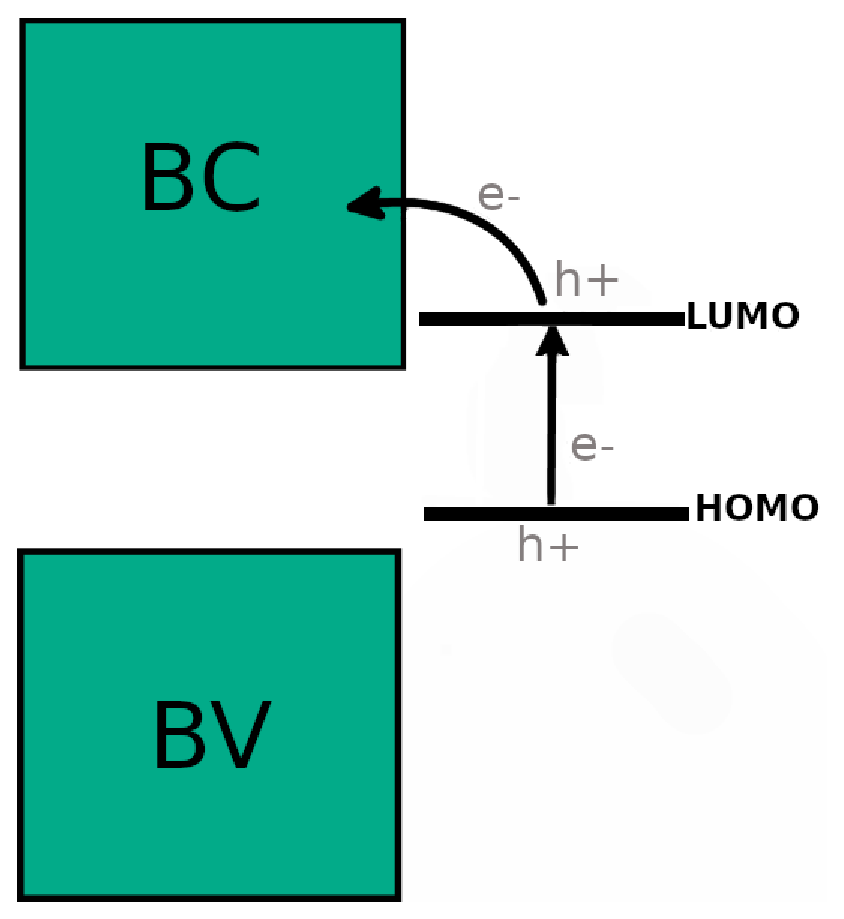
\includegraphics[height=7cm]{cap4/figs/fig_1_a_TUN_1.eps}
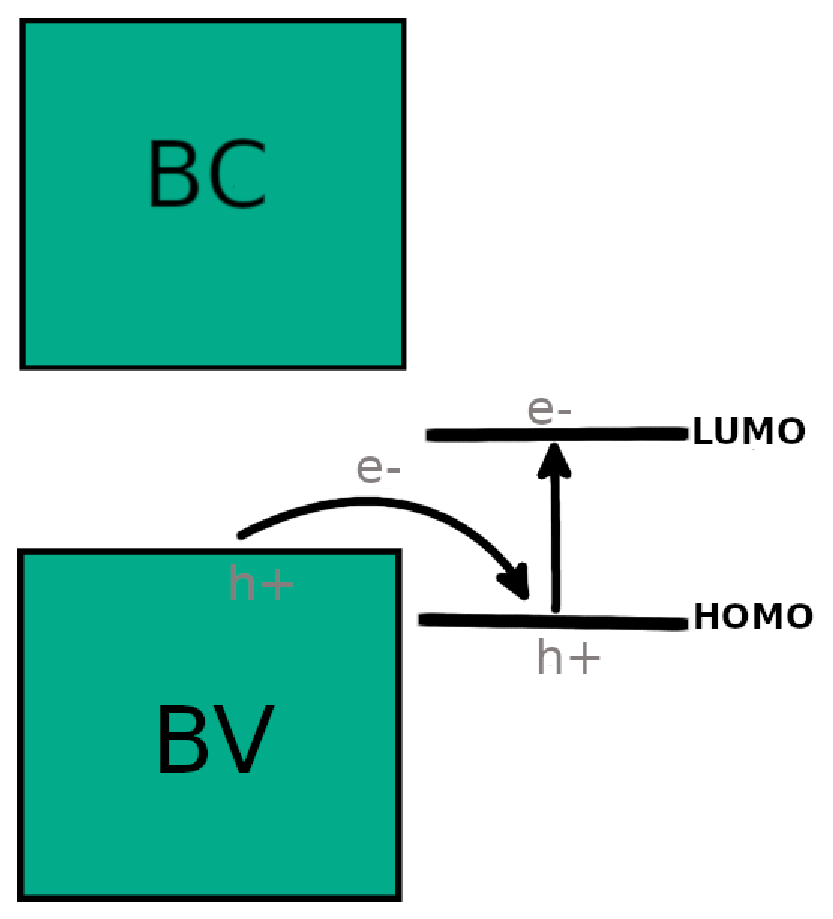
\includegraphics[height=7cm]{cap4/figs/fig_1_b_TUN_1.eps}
\caption{Sensibilización tipo n {\bf (izquierda)}, sensibilización tipo p {(\bf derecha)}}
\label{nyp}
\end{figure}

Para que el funcionamiento de una DSSC sea exitoso, todos los componentes deber ser seleccionados de manera que no sólo garanticen una buena eficiencia de la celda sino que también sean amigables con el medio ambiente y el costo de producción sea bajo en lo posible: el material del{\bf fotoelectrodo}, el {\bf colorante/sensibilizador} y el {\bf par redox}. 


En las DSSC de tipo n se utiliza generalmente dióxido de titanio en fase anatasa (TiO$_2$) como electrodo semiconductor de óxido metálico o fotoánodo debido a las ventajas del material sobre otros como su fácil síntesis, estabilidad, no toxicidad, bajo costo y también el amplio GAP en comparación con sus otras formas cristalinas ($3.2$ eV anatasa vs $3.0$ eV para rutilo)\cite{Hagfeldt2010}. En cambion, en las DSSC de tipo p, otros materiales son comúnmente utilizados para preparar fotocátodos: NiO\cite{Dini2016,Hod2013,Odobel2010}, AgCrO$_2$\cite{Xiong2015}, CuO\cite{Langmar2015,Jiang2016}, CuSCN\cite{Iwamoto2014,Chen2016}, Cu$_2$O\cite{Du2014} y CuAlO$_2$\cite{Miclau2017}. En particular, NiO se ha utilizado ampliamente en DSSC de este tipo debido a su estabilidad, amplio GAP ($3.6$–$4.0$) eV  y debido al potencial de la BV el cual es adecuado para que el proceso de transferencia de electrones del semiconductor al colorante ocurra ($0.54$ V frente a NHE a pH $7.30$)\cite{Odobel2010}.

El colorante, en ambos tipos de DSSC, debe tener ciertas características para un desempeño eficiente, esencialmente una absorción amplia y fuerte en el espectro visible y cercanas al IR para una mejor recolección de luz, estabilidad química, potencial redox apropiado de los orbitales HOMO y LUMO para que los procesos de inyección de carga y regeneración del colorante sean exitosos\cite{Sarkar2012}, fotoestabilidad y un grupo químicamente adsorbible para un acoplamiento fuerte con el semiconductor. Se han estudiado colorantes novedosos para aumentar la eficiencia dde la celda; para DSSC de tipo-n se han utilizado sensibilizadores a base de trifenilamina\cite{Fang2017,Jia2012,Li2015}, azo heterociclos\cite{Mahmood2014}, indolina\cite{Zhang2015}, triarilamina\cite{Wang2016}, carbazol\cite{Beni2015,Jia2012}, ditienilpirazina\cite{Godfroy2017}, coumarina\cite{Namuangruk2016,Feng2017,Han2017}, porfirina\cite{Birel2017,Mathew2014,Yella2011} y quinolinas\cite{Mao2016} mientras que en DSSC tipo-p colorantes a base de cumarina \cite{Daniel2017,Morandeira2008,Mizoguchi2008,Morandeira2005}, porfirina\cite{Palomaki2013,Borgstrom2005}, triarilamina\cite{Wild2016}, perileno diimidas \cite{Feihl2012,Chang2012}, isoindigo\cite{Ameline2015}, squaraina\cite{Warnan2014}, aril amina\cite{Yen2011}, carbazol\cite{Naik2017,Park2014}, etc.


En trabajos previos, nuestro grupo demostró sensibilización tipo n y tipo p en NP de TiO$_2$ anatasa\cite{Oviedo2012,Negre2012} y Ti$_{17}$O$_{24}$(OPri)$_{20}$ \cite{Negre2014}, respectivamente, por varios adsorbatos obteniendo una buena correlación con datos experimentales. Desarrollando más sobre la base de nuestra experiencia, en este capítulo mostramos cuán eficiente es el proceso de transferencia de carga en sistemas colorante-semiconductor cuando los mismos son iluminados con radiación de banda ancha. Para eso, estudiamos tres sistemas colorante-TiO$ _2 $ utilizando colorantes cuya estructura conjugada los convierte en buenos sensibilizadores para DSSC: (alizarina ({\bf ALZ})\cite {Oviedo2012} y catecol ({\bf CAT})\cite {Negre2012} y por otro lado, y {\bf FSD101}\cite {Fang2017}, ya que se han obtenido muy buenas eficiencias con colorantes que tienen triples enlaces en su estructura \cite {Yao2015, Mathew2014, Yella2011}. Además de calcular el espectro de los sistemas colorante-TiO$ _2 $ y reportar un análisis detallado del proceso de transferencia de carga fotoinducida en los diferentes complejos iluminados con una perturbación sintonizada con la energía del máximo del espectro, estudiamos la dinámica electrónica del sistema al iluminar con todas las longitudes de onda del espectro solar a nivel del mar y con estos resultados calculamos la eficiencia de la transferencia de carga colorante-NP fotoinducida. Todas las simulaciones aquí presentadas se basan en el modelo de enlaces fuertes del funcional de densidad dependiente del tiempo en tiempo real ({\bf RT-TD-DFTB}), que describe el sistema en condiciones de no equilibrio.

\begin{figure}[!htb]
\centering
  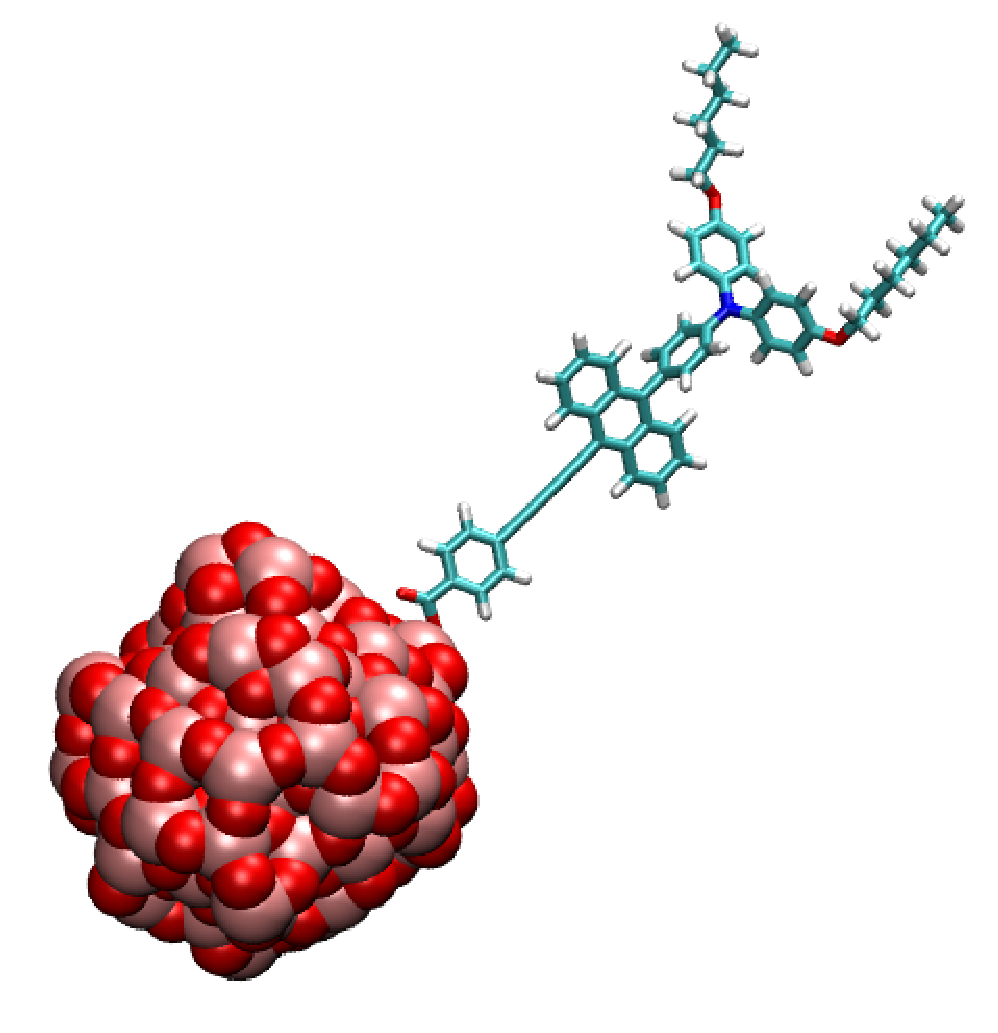
\includegraphics[width=0.50\linewidth]{cap4/figs/tpa_coords.eps}
  \caption{Estructura atómica del complejo FSD101-TiO$_2$}
  \label{FSD101}
\end{figure}


\newpage

\section{Espectros de absorción óptica}

Para todos los cálculos realizados en este capítulo, utilizamos un nanocluster anatasa de $270$ átomos ($90$ unidades de TiO$_2$, figura \ref{FSD101}) y {\bf ALZ}, {\bf CAT}  y {\bf FSD101} como colorantes sensibilizadores (figura \ref{compuestos}). Las estructuras de nanocluster de TiO$_2$ son las mismas que nuestro grupo describió anteriormente en el trabajo de Negre {\it et. al.} \cite{Negre2012} y se generaron a partir de simulaciones de dinámica molecular con LAMMPS a $300$K. La optimización de la geometría de los colorantes y de los complejos se realizaron utilizando el paquete dftb+ y se restringieron, en el segundo caso, a las coordenadas del sensibilizador y las cinco unidades de TiO$_2$ que se encuentran más cercanas al punto de unión del colorante.

\begin{figure}[!htb]
\centering
\subfloat[]{%
  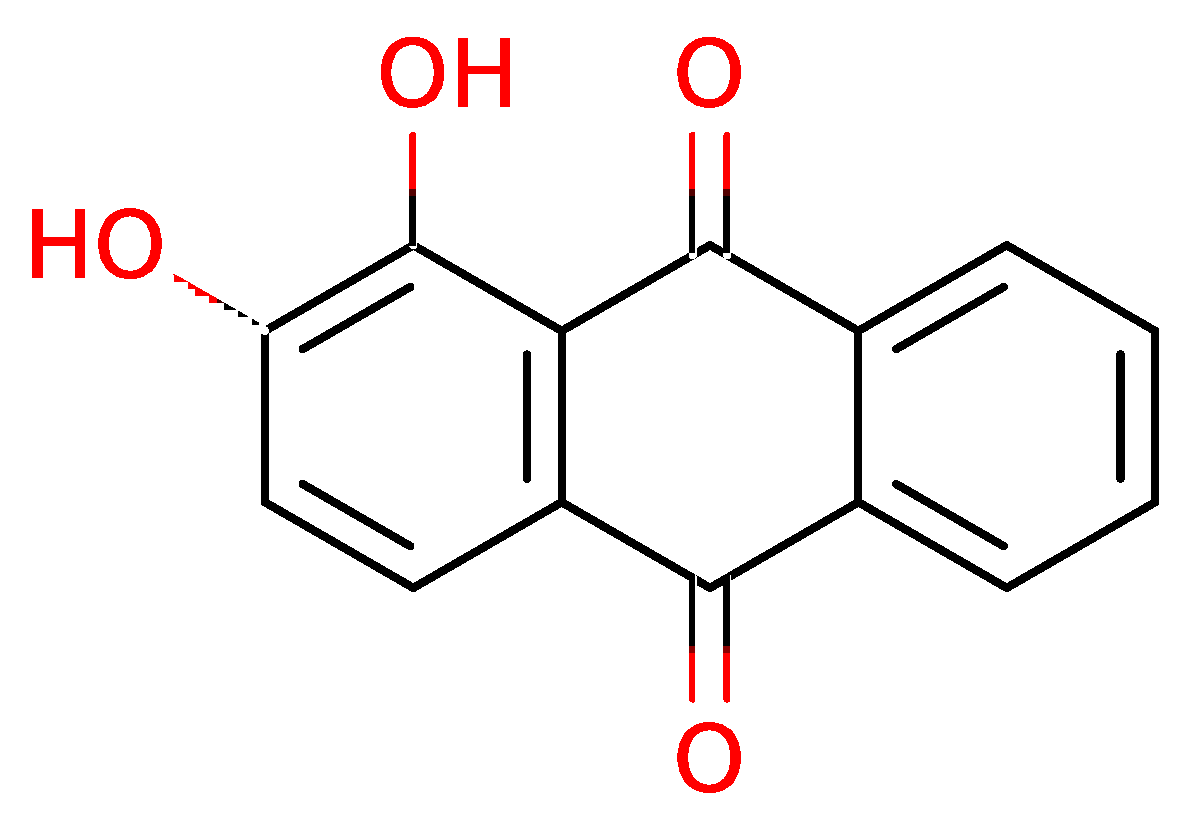
\includegraphics[width=0.3\linewidth]{cap4/figs/fig_3_a.eps}
  \label{alz}
}
\hspace{1.5cm}
\subfloat[]{%
  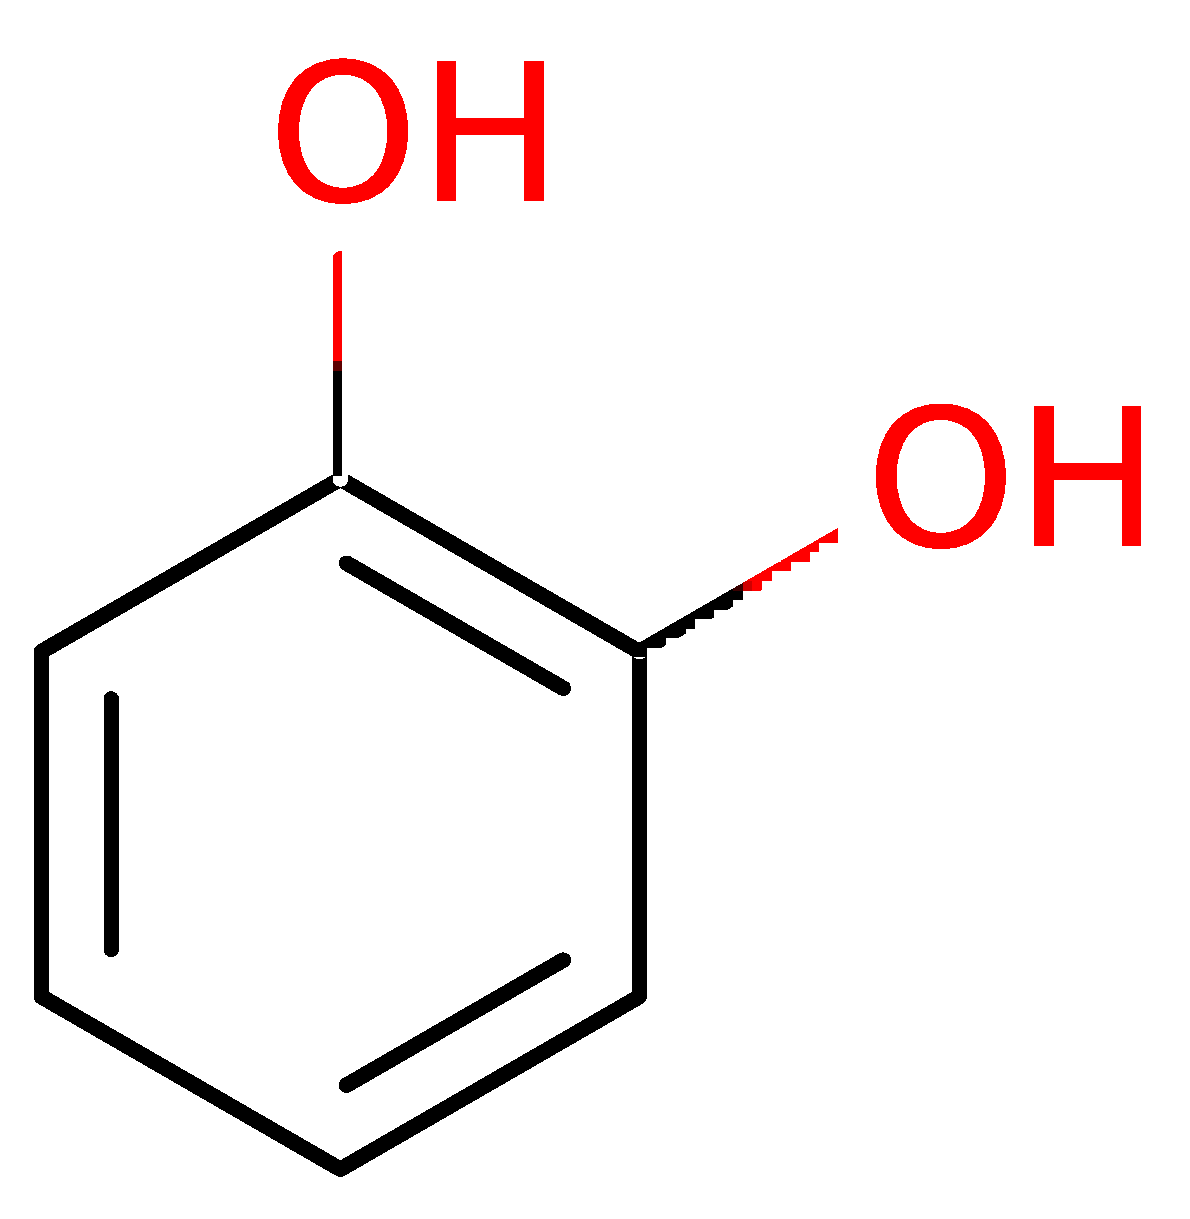
\includegraphics[width=0.15\linewidth]{cap4/figs/fig_3_b.eps}
 \label{cat}
}
\hspace{1cm}
\subfloat[]{%
  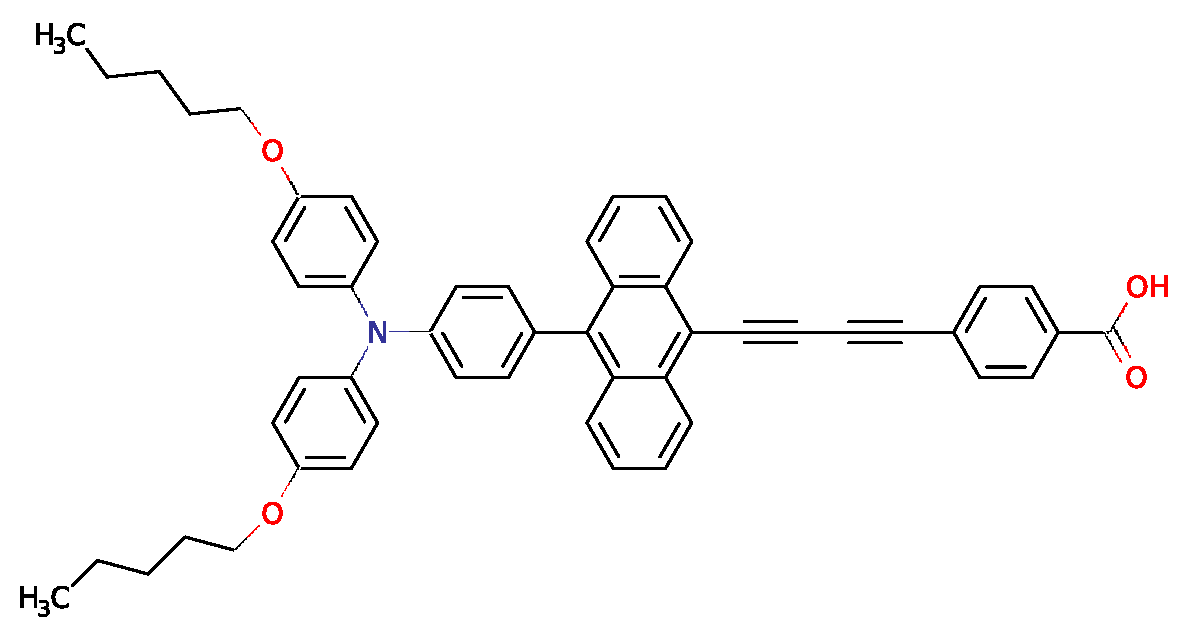
\includegraphics[width=0.8\textwidth]{cap4/figs/fig_3_c.eps}
 \label{fsd101}
}
\caption{Compuestos estudiados: {\bf (a)} ALZ, {\bf (b)} CAT y {\bf (c)} FSD101}
\label{compuestos}
\end{figure}


En la tabla \ref{tabla_maximos} se comparan las energías de absorción ({\bf E$_{ab}$}) obtenidas teóricamente con TD-DFTB y experimentalmente de literatura, tanto para colorantes libres como para los complejos colorante-NP. Es importante mencionar que los espectros de absorción de los sensibilizadores y complejos medidos experimentalmente se registraron en disolventes orgánicos, mientras que nuestros resultados corresponden al sistema en vacío y que los valores tabulados corresponden a la energía de excitación más baja en cada caso.


\hspace{1.5cm}

%\begin{table}[h]
%  \caption{Energías de absorción ({\bf E$_{ab}$}) para las excitaciones de más baja energía (en eV) para colorantes libres y sistemas colorante-NP, obtenidos por el método TD-DFTB (en vacío) y valores experimentales encontrados en literatura}
%  \label{tabla_maximos}
%  \centering
%  \resizebox{14cm}{!} {
%  \begin{tabular}{ c  c  c  c  c }
%   \hline
%   \multicolumn{1}{c}{} & \multicolumn{2}{c}{E$_{ab}$ colorante libre / eV} & \multicolumn{2}{c}{E$_{ab}$ colorante adsorbido / eV} \\
%   \hline
%    Colorante & TD-DFTB & experimental &  TD-DFTB & experimental \\
%   \hline
%    ALZ & $2.85$ & $2.88\cite{Huber2000}$ & $2.44$ & $2.48\cite{Huber2000}$\\
%    CAT & $4.55$ & $4.43\cite{Wang2003}$ & $3.00$ & $3.18\cite{Wang2003}$\\ 
%    FSD101 & $2.40$ & $2.77\cite{Fang2017}$ & $2.43$ & $2.89\cite{Fang2017}$\\ 
%    \hline
% \end{tabular}
% }
%  \end{table}
  
 
\hspace{1.5cm} 

En primer lugar, observamos que ambos valores absolutos de las E$_{ab}$ concuerdan en general, de forma cualitativa e incluso cuantitativamente para ALZ. Los valores de las energías cambian tras la absorción de los colorantes CAT y ALZ a excepción de FSD101 en donde el cambio es muy pequeño. La aparición de una nueva banda de absorción cuando se une CAT en la NP coindice con los datos encontrados en literatura. En cuanto a las relaciones de absorción entre el colorante libre y las bandas de colorante adsorbido, en general, concuerdan cualitativamente con los datos experimentales. En el caso de la molecula FSD101, aunque el máximo de absorción aumente con la adsorción tanto teórica como experimentalmente, en el caso segundo caso, el aumento es mayor. 


De estudios previos \cite{Oviedo2012, Negre2012} se sabe que ALZ es una molécula que exhibe un mecanismo de inyección indirecto (tipo I) mientras que CAT exhibe un mecanismo directo (tipo II) para la inyección de electrones. Estos trabajos sugieren que es posible predecir el mecanismo de inyección electrónica de los complejos, analizando y comparando los espectros de absorción del colorante y la NP aislados con respecto al espectro del sistema colorante-TiO$_2$. 
En los espectros del sistema ALZ-NP (figura \ref{alz_spec}), se puede observar que la banda de menor energía sufre un corrimiento hacia el rojo junto con la adsorción de la molécula sobre la NP de TiO$_2$, sin embargo, no aparece una nueva banda en la región visible cuando esto ocurre. El sistema CAT-NP (figura \ref{cat_spec}) muestra la aparición de una nueva banda de transición a $3.00$ eV cuando se produce la unión del colorante con la NP y por último, en el caso de FSD101-NP (figura \ref{fsd101_spec}), los espectros no muestran un cambio significativo para la banda de menor energía ni la aparición de nuevas bandas cuando el colorante está adsorbido en el semiconductor por lo que el mecanismo de inyección electrónica es indirecto.

\begin{figure}[!htb]
\centering
\subfloat[]{%
  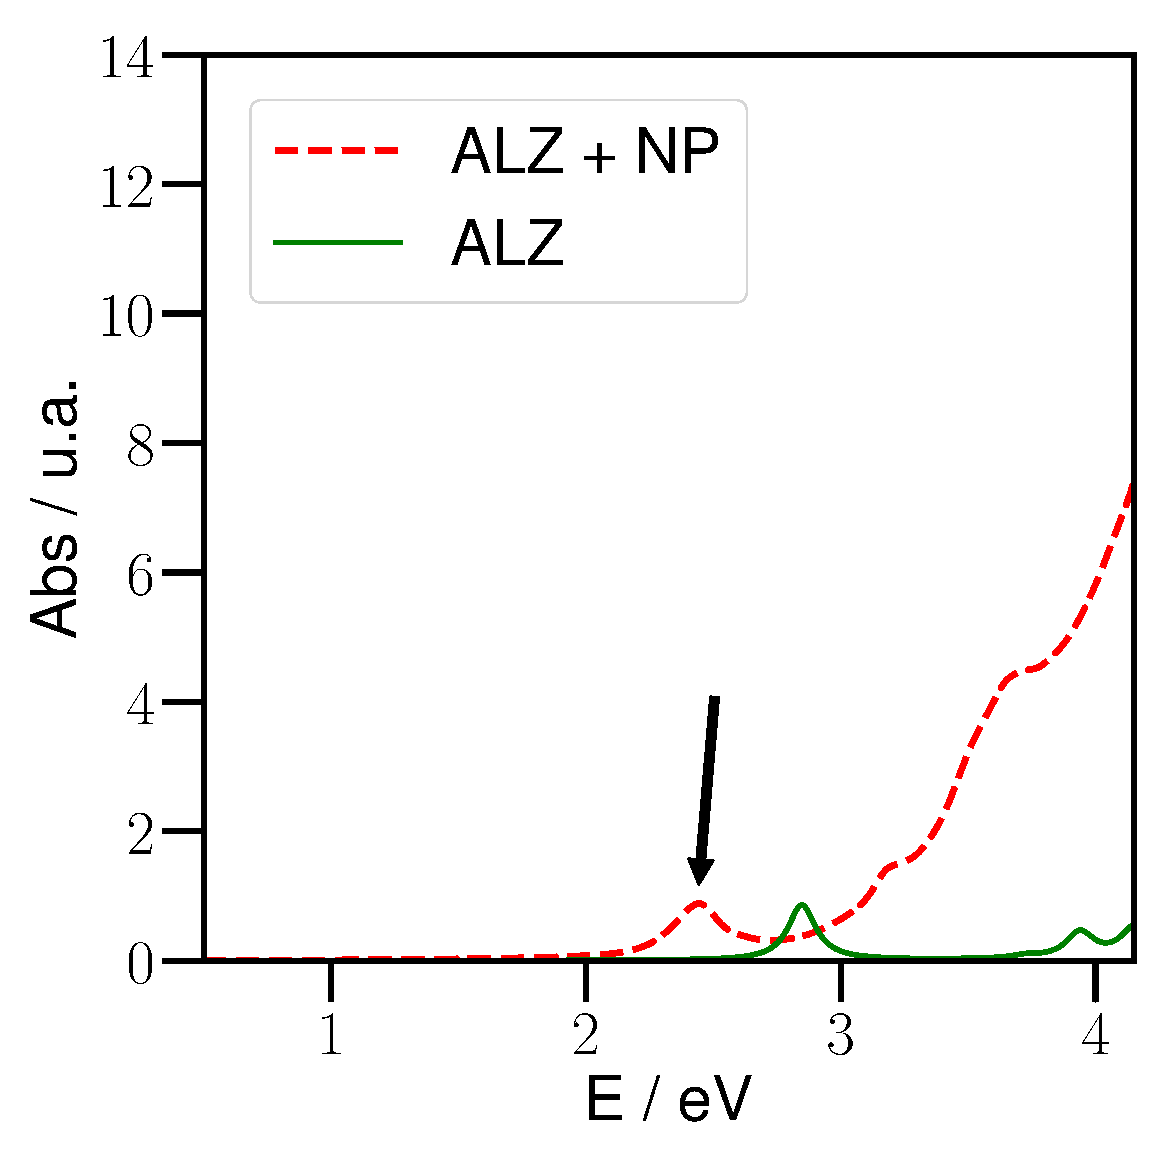
\includegraphics[width=0.32\linewidth]{cap4/figs/spec_alz.eps}
  \label{alz_spec}
}
\subfloat[]{%
  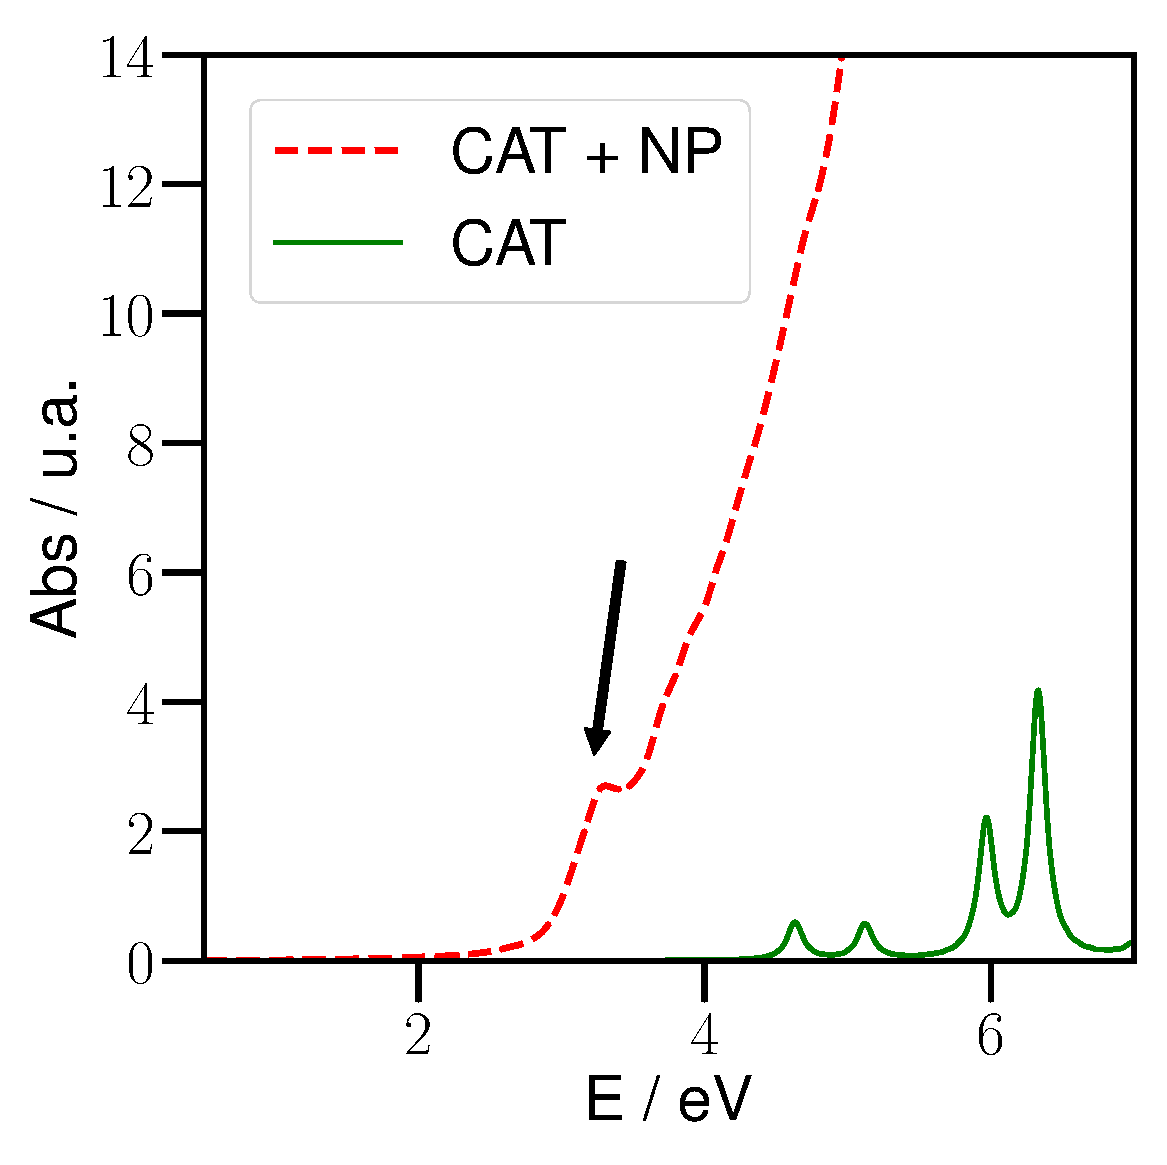
\includegraphics[width=0.32\linewidth]{cap4/figs/spec_cat.eps}
  \label{cat_spec}
}
\subfloat[]{%
  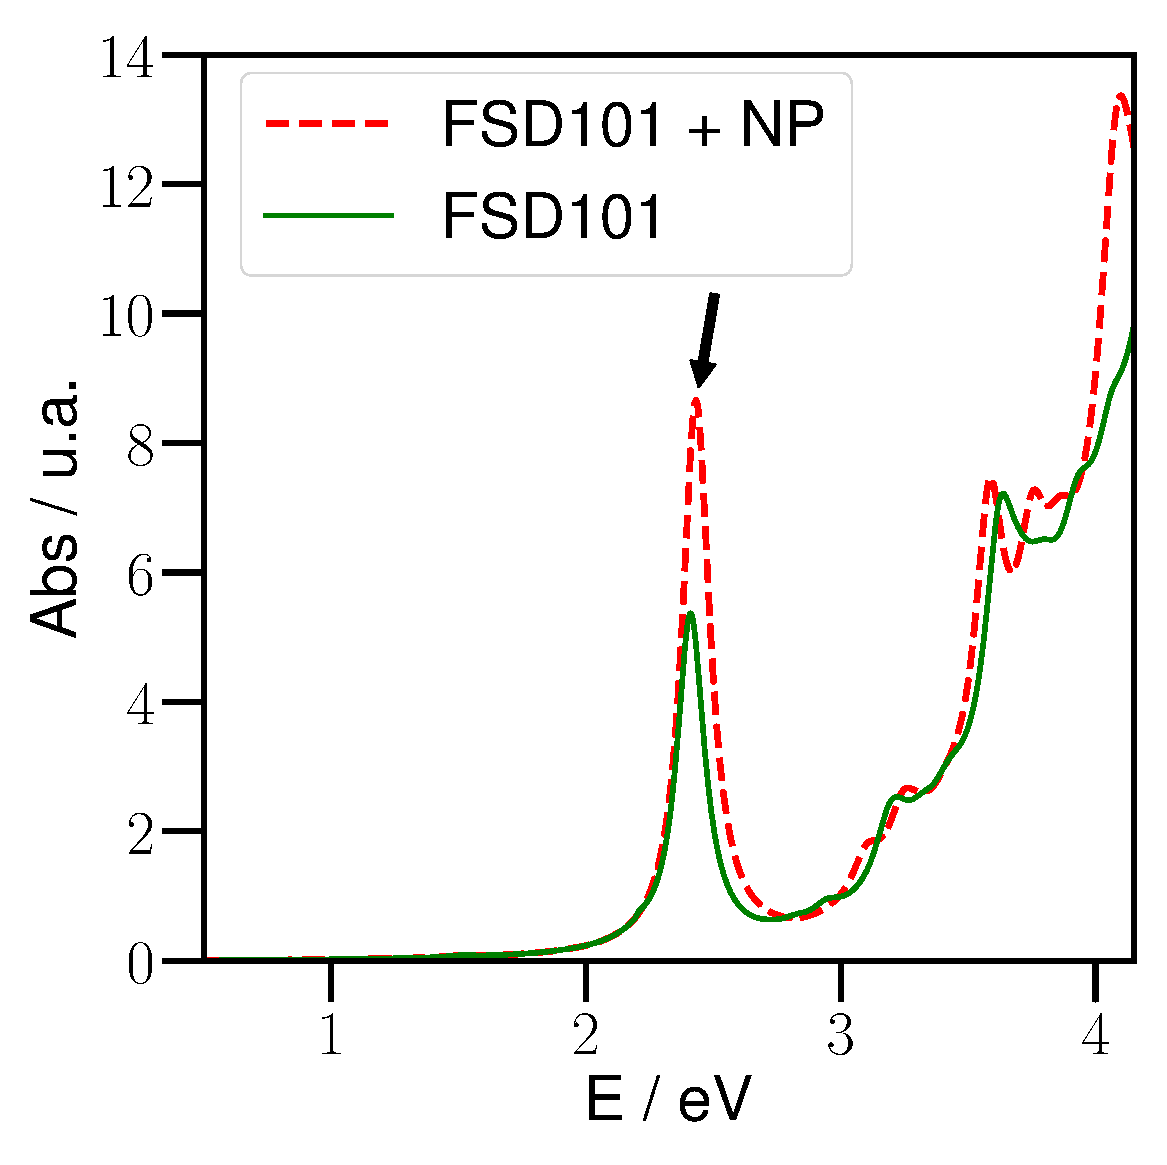
\includegraphics[width=0.32\textwidth]{cap4/figs/spec_fsd101.eps}
  \label{fsd101_spec}
}
\caption{Superposición de los espectros ópticos de colorantes aislados y colorantes adsorbidos en la NP de TiO$_2$, {\bf (a)} ALZ, {\bf (b)} CAT y {\bf (c)} FSD101}
\label{espectros}
\end{figure}


\vspace{1.5cm} 


\section{Transferencia de carga}


La figura \ref{transferencia_carga} muestra la evolución de la distribución de carga dependiente del tiempo en el colorante y la NP tras la fotoexcitación del complejo colorante-TiO$_2$ con una perturbación sinusoidal del campo eléctrico dependiente del tiempo con la frecuencia de la banda de absorción de energía más baja de cada espectro: $2.44$ eV para ALZ + NP, $3.00$ eV para CAT + NP y $2.43$ eV para FSD101 + NP (ver flechas de la figura \ref{espectros}), y con dirección del momento dipolar de transición del sistema total. En general, en la figura \ref{transferencia_carga} se puede observar que existe una transferencia neta de carga en todos los sistemas. Las moléculas CAT y FSD101 se cargan positivamente a medida que aumenta el tiempo, mientras que la NP, en ambos sistemas, se carga negativamente. Estos resultados indican que con la fotoexcitación del colorante en su máxima absorción, la carga se transfiere del colorante a la BC de la NP, proceso que induce inyección de electrones. En el caso de ALZ, la molécula se carga negativamente en conjunto con la evolución temporal, mientras que el SC adquiere una carga positiva. La carga en este sistema se transfiere desde la BV del SC al HOMO de la molécula, en contraste con los otros colorantes estudiados y por lo tanto se observa inyección de huecos.


\begin{figure}[!htb]
\centering
\subfloat[]{%
  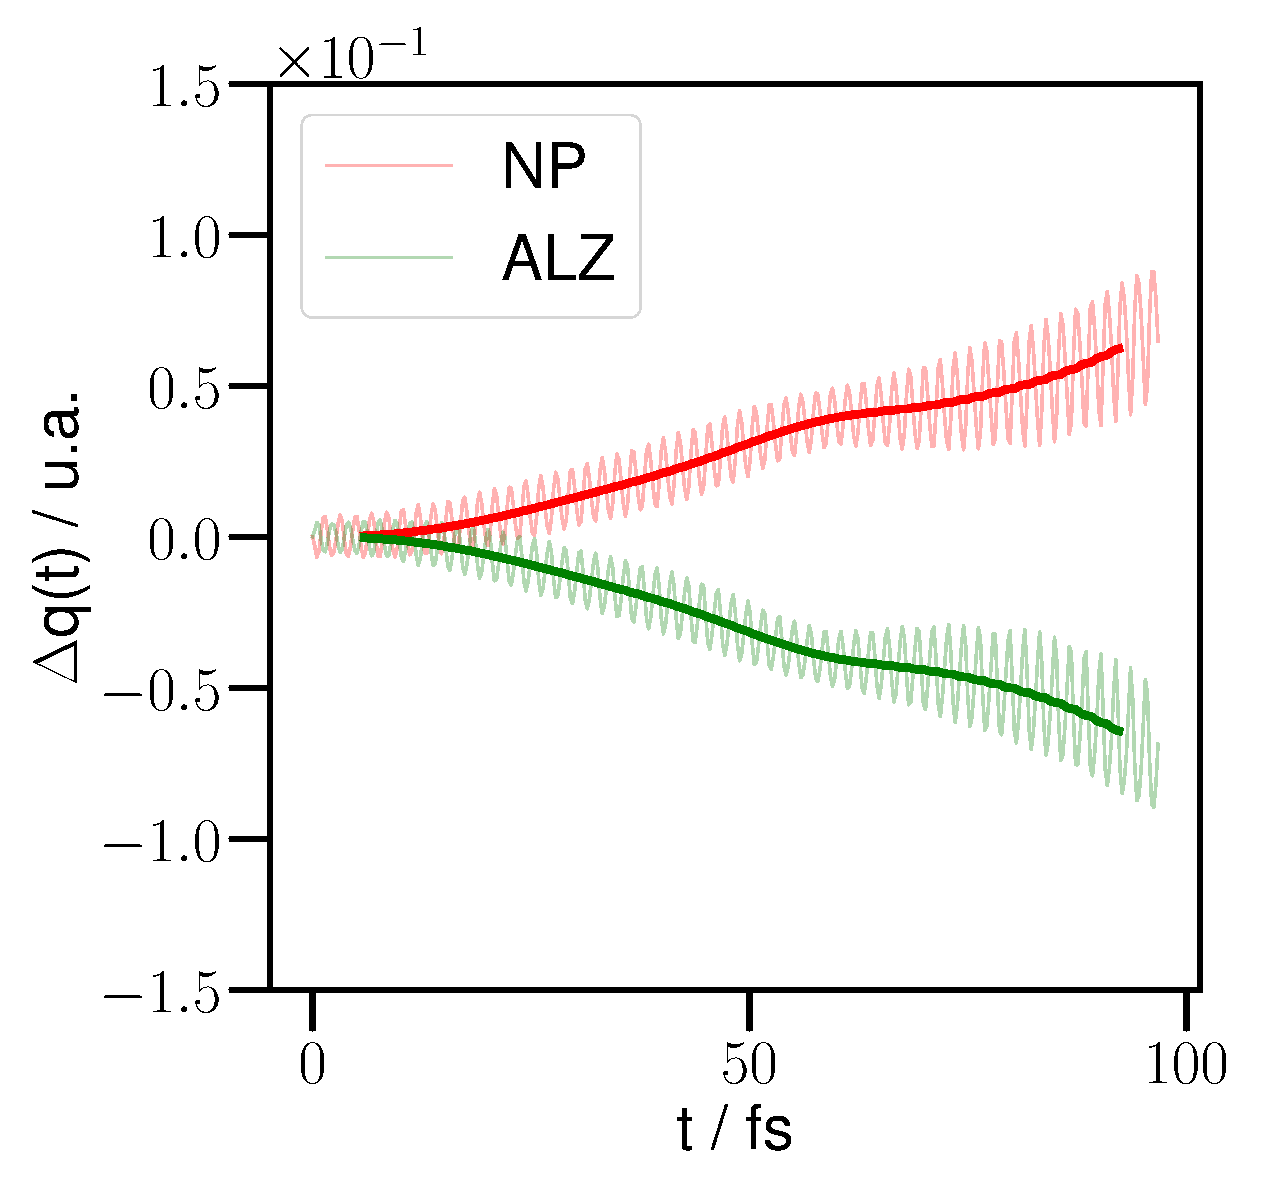
\includegraphics[width=0.32\linewidth]{cap4/figs/cargas_alz.eps}
  \label{alz_q}
}
\subfloat[]{%
  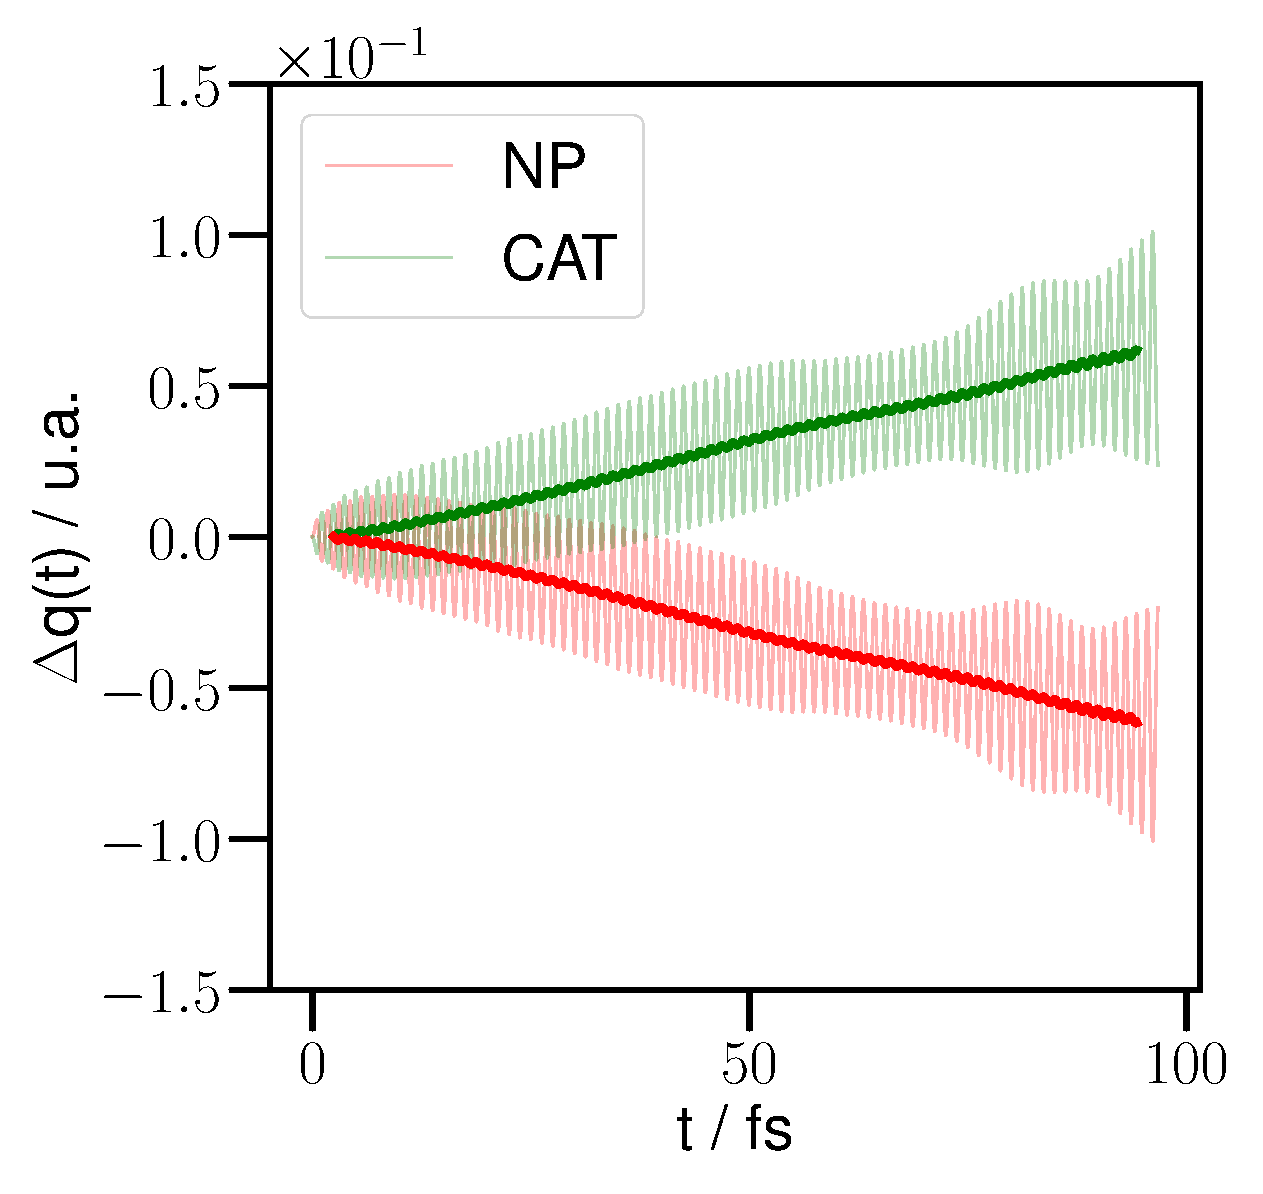
\includegraphics[width=0.32\linewidth]{cap4/figs/cargas_cat.eps}
  \label{cat_q}
}
\subfloat[]{%
  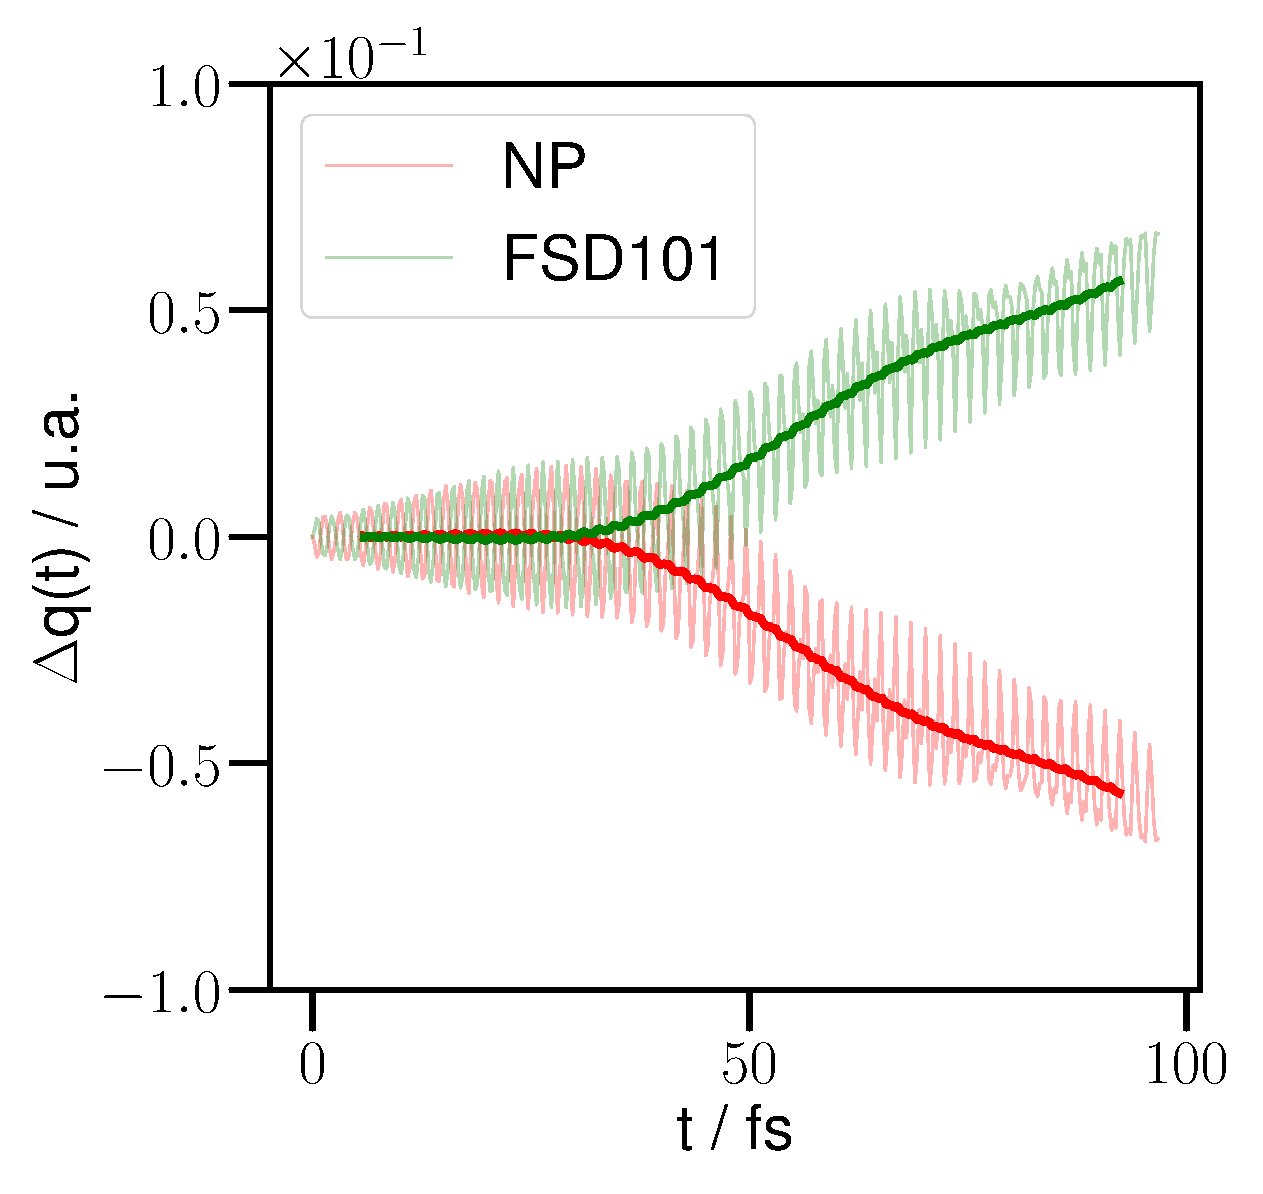
\includegraphics[width=0.32\textwidth]{cap4/figs/cargas_fsd101.eps}
  \label{fsd101_q}
}
\caption{Evolución de la carga durante las simulaciones de inyección electrónica para iluminaciones a $2.44$ eV para ALZ + TiO$_2$ {\bf (a)}, a $3.00$ eV para CAT + TiO$_2$ {\bf (b)} y a $2.43$ eV para FSD101 + TiO$_2$ {\bf (c)}}
\label{transferencia_carga}
\end{figure}


\newpage

\subsection{Eficiencia de la transferencia de carga}

\begin{figure}[!htb]
\centering
\subfloat[]{%
  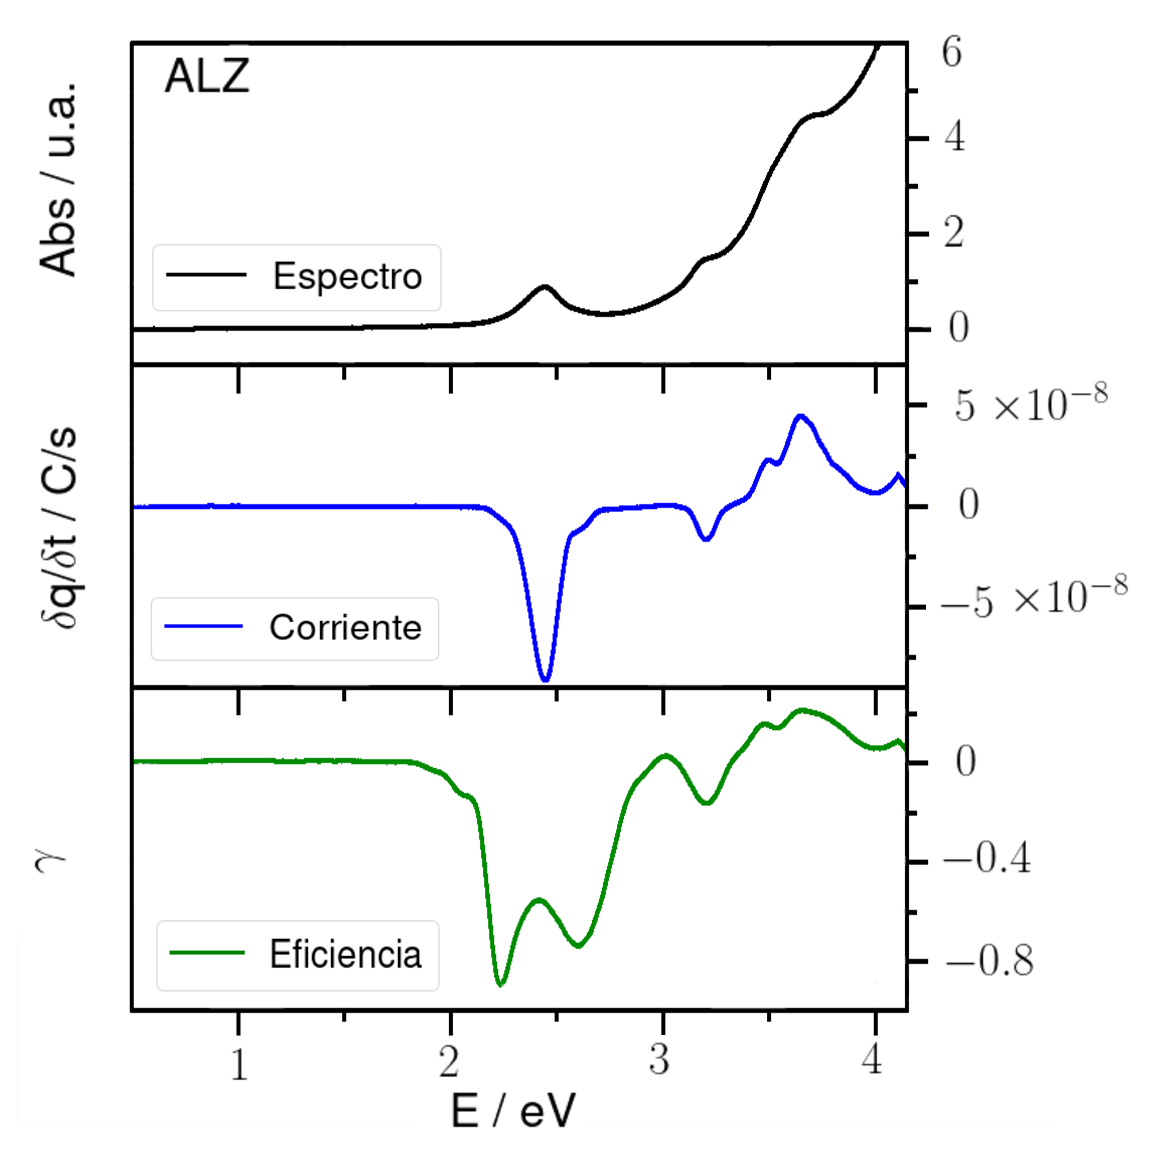
\includegraphics[width=0.45\linewidth]{cap4/figs/imagen1.eps}
  \label{alz_c}
}
\subfloat[]{%
  \includegraphics[width=0.45\linewidth]{cap4/figs/imagen2.eps}
  \label{cat_c}
}
\hspace{1cm}
\subfloat[]{%
  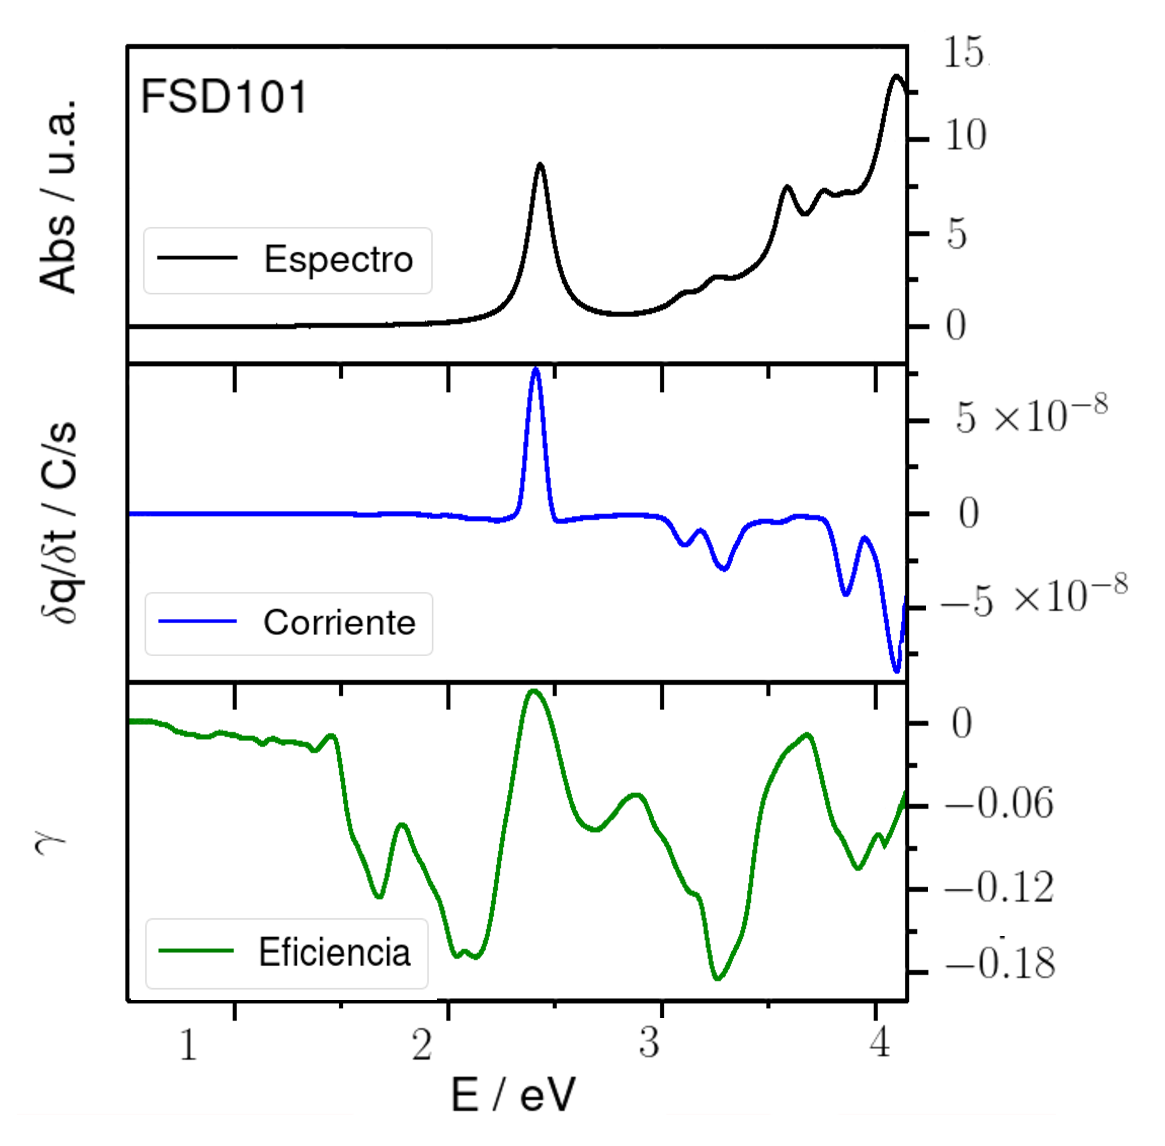
\includegraphics[width=0.45\textwidth]{cap4/figs/imagen3.eps}
  \label{fsd101_c}
}
\caption{Espectros de absorción para los sistemas colorante-TiO$_2$ comparados con las pendientes de los promedios de las cargas dependientes del tiempo y la eficiencia del proceso de transferencia de carga entre el colorante y la NP ($\gamma$) para ALZ {\bf (a)}, CAT {\bf (b)} y FSD101 {\bf (c)} en función de la energía ({\bf E}). Los valores positivos en las pendientes y las eficiencias corresponden a transferencia de electrones desde el colorante a la NP, mientras que valores negativos indican transferencia de huecos.}
\label{corriente}
\end{figure}


La figura \ref{corriente} muestra los espectros de absorción de los complejos, los valores de corriente de transferencia de carga promedio en una ventana de simulación de $100$ fs y la eficiencia del proceso de inyección de carga. Estos últimos valores se obtuvieron calculando la pendiente de la carga con respecto al tiempo para cada una de las energías analizadas en la ventana de simulación, es decir, sintonizando láseres con ondas sinusoidales con longitudes de onda que se encuentran dentro del espectro solar a nivel del mar: ($300-2500$) nm o ($0.5-4.15$) eV. La energía absorbida (utilizada como entrada para el cálculo de la eficiencia) se calculó de la misma manera, a partir de la potencia calculada como la pendiente obtenida al ajustar la energía total del sistema en función del tiempo dentro de la ventana de simulación. En todos los casos, tanto la carga transferida como la energía total son lineales en el tiempo, dentro de la ventana, lo cual coincide con el hecho de que las simulaciones se realizan dentro del régimen de respuesta lineal.

% %%% CORRIENTE
% 
Los valores de corriente obtenidos para CAT-TiO$_2$ (figura \ref{cat_c})son positivos en todas las longitudes de onda incidentes y se observa una corriente máxima (positiva) a $3.00$ eV. Este valor es el mismo que se obtuvo como máxima absorción del espectro de absorción óptica. El hecho de que el valor máximo de la corriente obtenida en función de las cargas del colorante sea positivo y se observe como consecuencia de iluminar el sistema con la longitud de onda de absorción máxima indica transferencia de electrones, lo cual concuerda con los resultados de trabajos previos \cite{Negre2012}. Para los otros dos colorantes, los valores positivos y negativos de la corriente promedio en los gráficos de la figura \ref{alz_c} y \ref{fsd101_c} indican la existencia de dos direcciones de inyección diferentes que operan en diferentes longitudes de onda dentro del espectro solar. Para ALZ-TiO$_2$ (figura \ref{alz_c}) en el rango ($1.8-3.32$) eV se observa transferencia de huecos y de $3.32$ eV a $4.15$ eV transferencia de electrones. En este caso, también se observa una corriente máxima en la absorción máxima a $2.44$ eV pero el valor es negativo, lo que significa que la molécula se carga negativamente en el tiempo, lo cual corresponde a un proceso de transferencia de huecos. En el gráfico de corriente de FSD101-TiO$_2$ (figura \ref{fsd101_c}), se observa transferencia de huecos en los intervalos ($1.8-2.3$) eV y ($2.5-4.15$) eV y transferencia de electrones en el intervalo ($2.3-2.5$) eV. La corriente es máxima cuando el sistema se ilumina con la longitud de onda del máximo de absorción a $2.43$ eV y muestra transferencia de electrones como el complejo CAT-TiO$_2$. En la figura \ref{corriente} también se observa que cuando se ilumina a energías más altas o longitudes de onda más cortas, que corresponde a la banda de absorción del NP (ver los espectros de absorción, figura \ref{espectros}) para ALZ-TiO$_2$ y FSD101-TiO$_2$ la carga se transfiere en sentido opuesto al obtenido al iluminarse con la energía que absorbe el colorante y este comportamiento no se observa para CAT-TiO$_2$. Finalmente, también se puede ver en la figura \ref{espectros} que los gráficos de corriente promedio revelan más información sobre las bandas de absorción del colorante en el sistema, con respecto al espectro de absorción y que muchas características se pueden determinar dentro del rango de absorción donde la banda de la NP domina el espectro. 

Es una característica general de todos los sistemas estudiados que la transferencia de huecos ocurre solo por encima de un cierto umbral de energía. Esto se puede racionalizar en términos de los diagramas que se muestran en la figura \ref{transferencia_carga}. Las transiciones de energía más bajas son todas del tipo que se muestra en el gráfico de la izquierda de la figura \ref{nyp} a excepción de CAT para el que la transición energética más baja corresponde a la situación mostrada en el gráfico derecho de la misma figura. A medida que aumenta la energía de excitación, se promueven electrones de orbitales por debajo del HOMO, que deben solaparse con más fuerza con la BV de la NP para mostrar transferencia de huecos.
% 
% %%EFICIENCIA
% 
La eficiencia del proceso de transferencia de carga entre el colorante y la NP, ($\gamma$), se calculó para cada energía a partir de la relación entre el flujo de fotones absorbidos y el número de portadores de carga recolectados. Para obtener el número de fotones por segundo, se calculó la potencia absorbida en cada frecuencia como la pendiente de la energía en función del tiempo (como se mencionó anteriormente), mientras que los valores del número de portadores de carga se obtuvieron a partir de las corrientes promedio obtenidas previamente. Los resultados de la eficiencia se muestran en la figura \ref{corriente}.


Para el sistema ALZ-TiO$_2$ se observa un pico máximo a $2.23$ eV con $\gamma= -0.89$, como el valor obtenido es negativo en este complejo, la mayor eficiencia del proceso de transferencia de carga se observa cuando se inyectan electrones de la BV en el colorante. 


En cambio, para CAT-TiO$_2$, se observa un pico con $\gamma = 1.7$ a $3.00$ eV y se inyectan electrones desde el colorante a la BC. En este caso, a diferencia del complejo con ALZ como colorante, la energía de absorción máxima coincide con la energía del valor más alto de $\gamma$. El hecho de que la eficiencia tenga un valor superior a 1 para este sistema se puede atribuir al mecanismo de inyección directa. Como hemos descrito en trabajos anteriores \cite{Oviedo2012}, es apropiado un enfoque de la teoría de perturbaciones de primer orden en el que la población inyectada en el LUMO escapa a una velocidad constante al CB. Entonces, la energía que ingresa se utiliza para bombear electrones desde el HOMO al LUMO, que luego escapan a múltiples estados de la CB de una manera incoherente y adiabática (sin inversión de energía) caracterizada por una constante de velocidad simple. De esta manera, se puede obtener una gran eficiencia si la población del LUMO se mantiene en un estado estable, invirtiendo una pequeña cantidad de energía solo para promover electrones que luego se transfieren adiabáticamente sin costo adicional de energía. 

Para FSD101-TiO$_2$ se observa una eficiencia máxima de $\gamma = -0.18$ para una iluminación de alrededor $3.26$ eV, dada por la transferencia de huecos. Por otro lado, a energías inferiores a $2.30$ eV se logra una gran eficiencia en una zona del espectro para la cual no se puede observar transferencia de carga ni absorción de energía apreciables. Un comportamiento similar ocurre para el caso de ALZ-TiO$_2$, donde las eficiencias máximas corresponden a los lados de la banda de absorción principal a $2.33$ eV. 

En los complejos CAT-TiO$_2$ y FSD101-TiO$_2$, el acoplamiento de los colorantes a los estados de la NP es menor que en CAT-TiO$_2$ como se puede inferir de los espectros de absorción mostrados en la figura \ref{espectros}. El acoplamiento de ALZ se puede caracterizar como intermedio entre CAT y FSD101, ya que existe una pequeña superposición espectral entre el borde de absorción del NP y el colorante y se observa una renormalización de la excitación de aproximadamente $0.3$ eV. El acoplamiento de FSD101 es el más bajo de los tres casos estudiados, debido a la pequeña renormalización de la energía y la pequeña superposición espectral. En los casos en los que el acoplamiento es chico, no se puede asumir que en el régimen resonante la población del orbital LUMO del colorante se encuentra en un estado estable, ya que el acoplamiento no es lo suficientemente fuerte como para expulsar la carga del LUMO a la misma velocidad con la que es bombeada por el campo externo. Por lo tanto, se muestra que en los casos de resonancia, es decir ALZ-TiO$_2$ y FSD101-TiO$_2$, la eficiencia no es máxima. Se logran eficiencias más altas en zonas del espectro que muestran una pequeña absorción y, a su vez, una transferencia de carga no despreciable. En estas situaciones, dado que la velocidad de población del LUMO es pequeña, incluso un pequeño acoplamiento a la NP puede forzar a que la población bombeada se transfiera y el sistema se encuentre en un régimen similar al descrito anteriormente.


\subsection{Cálculos de respuesta lineal}

\begin{figure}[h!]
\centering
  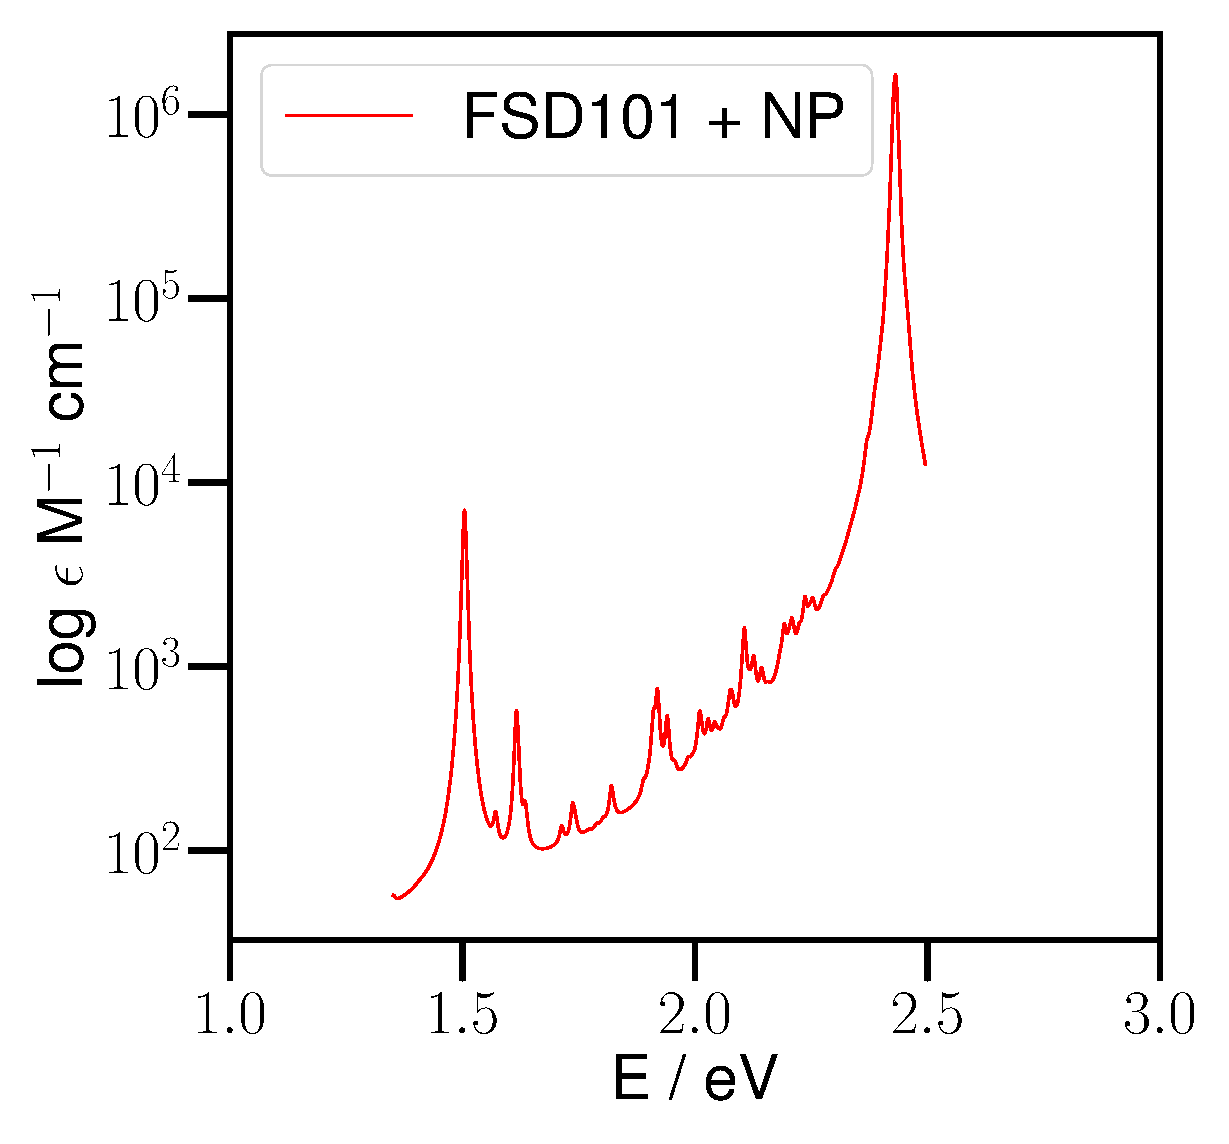
\includegraphics[height=8cm]{cap4/figs/rta_lineal.eps}
  \caption{Espectro de respuesta lineal para el sistema FSD101+ NP: logaritmo del coeficiente molar de extinción ($\epsilon$) en función de la energía ({\bf E})}
  \label{rta_lineal}
\end{figure}

En la figura \ref{corriente} se observa que el sistema FSD101-NP en el rango de energías ($0.5-2.0$) eV no muestra absorción ni corriente apreciable en la escala mostrada, sin embargo, la eficiencia global de transferencia de carga es apreciable. 

Para justificar estos resultados obtenidos realizamos cálculos a nivel DFTB dependiente del tiempo basado en la teoría de respuesta lineal implementado en el paquete dftb$^+$ \cite{Niehaus2001}. Esta herramienta es muy importante ya que nos permitió constatar que efectivamente hay absorción a partir de $1.5$ eV  y en el rango que nos interesa (ver figura \ref{rta_lineal}) a pesar de que en los gráficos que se mostraron anteriormente no se pudo apreciar dicha absorción pero está presente e influye en el valor final de eficiencia. Con estos resultados, corroboramos que los valores obtenidos de eficiencia tienen sentido.

% 
% 
 \section{Conclusiones}


Los espectros de absorción óptica, además de mostrar una buena concordancia con los datos experimentales, revelan los mecanismos de inyección electrónica de cada uno de los sistemas: CAT-TiO$_2$ presenta mecanismo tipo II (o directo) mientras que ALZ-TiO$_2$ y FSD101-TiO$_2$ presenta un mecanismo de tipo I (o indirecto).
 
Iluminando con la energía del máximo de absorción observamos transferencia de carga en los tres complejos. En CAT-TiO$_2$ y FSD101-TiO$_2$ la inyección electrónica ocurre desde el colorante a la NP, mientras que en ALZ-TiO$_2$ la transferencia de carga ocurre desde la NP al colorante.

Las principales conclusiones de este capítulo están relacionadas con los resultados obtenidos del estudio del sistema bajo iluminación sobre una amplia banda de energías, correspondiente a todo el ancho del espectro solar. En este caso observamos que para el complejo con CAT solo hay transferencia de electrones en todo el rango mientras que con los otros sistemas, dependiendo de la energía incidente, puede haber transferencia de huecos o electrones. Finalmente, con el análisis de las eficiencias se observó que la mayor eficiencia del proceso primario de transferencia de carga no ocurre necesariamente al iluminar en el máximo de absorción. Además, la eficiencia global de la transferencia de carga está dada por un compromiso entre la transferencia de huecos y de electrones. Para ALZ-TiO$_2 $ y FSD101-TiO$_2$ la mayor eficiencia ocurre por transferencia de huecos y no con la energía de máxima absorción. En CAT-TiO$_2$, la mayor eficiencia viene dada por la transferencia de electrones con la energía del máximo de absorción.



